% !TEX root = ../thesis.tex
% !TeX spellcheck = en_US

This chapter covers the design of the implemented hybrid routing algorithm.
First, the overall context is presenting specifically the requirements and constrains of the algorithm.
Second, details on the decisions regarding the routing strategy and general design are presented.
Finally, an overview of the separate components is given as well as a description on the deployment of this algorithm.

\section{Requirements and constrains}

	% Used by agents for wayfinding
	The primary goal of the hybrid routing algorithm is to provide a path planning algorithm that is integrated into the MARS framework and offers more accurate paths compared to common graph based algorithms on road datasets, thus, enhancing agent based simulations.
	Such a major goal implies several constrains on the architecture and design of the software.
	
	\subsection{Requirements}
	
		Functional requirements of the resulting software can be formulated quite easily, since this is not a large commercial product.
		The hybrid routing algorithm should determine an optimal path between two locations following ways and traversing open spaces while avoiding obstacles.
		A configurable weight function should be used to assign a weight to each edge in order to find the path with the minimum weight.
		Processing of geospatial data must consider existing road network data as well as obstacles, which are features that will be avoided on paths traversing open spaces.
		It must be possible for the shortest path to alternate between segments following roads and open spaces.
		
		More complex and time consuming are the quality requirements.
		Because this is not part of a commercial software development, these requirements are not part of any tender and were not even formulated.
		Nonetheless, they exist and consist of the following aspects.
	
		The largest quality requirement in terms of effort is performance.
		It affects large parts of the software architecture since the resulting algorithm, despite its complexity, should ideally have a negligible impact on the overall performance of a simulation compared to current graph based routing approaches.
		Routing algorithms and engines often consist of two steps: preprocessing and answering routing queries.
		In order to create fluent and fast simulations, the performance of answering numerous routing requests must be as good as possible.
		The time needed for preprocessing is of less importance.
		
		A rather obvious requirement is the correctness of resulting routes.
		Answers of routing queries must return the shortest route according to a given weight function.
%		Even when using an approximation algorithm to determine shortest paths, the results can be checked against all other possible paths to verify the optimality of the resulting path.
		
		Another quality requirement is the closeness of the resulting routes to real pedestrian behavior.
		Unfortunately, this can hardly be measured without having extensive data of real world pedestrians in real world locations.
		Ideally, the trajectory of a calculated route should be identical to a real world pedestrian trajectory.
		It should at least make sense to an observer without additional knowledge of the real world location.
		The coordinates of waypoint on the calculated and on real trajectories must not be exactly the same, since real pedestrian behavior is not part of the shortest path calculations but is instead a task for realistic agent modeling.
		Such behavior includes for example a typical minimum distance kept to obstacles or a minimum radius of walked curves.

		Next to the domain specific requirement, the overall code itself should of course be well documented and tested.
	
	\subsection{Constrains}
	\label{subsec:constrains}
		
		% Well integrated into MARS and NTS, no new dependencies
		One major constraint is the integration of final algorithm into the \term*{MARS} framework to make the use as easy as possible and to centralize the code base for better maintenance.
		This means the programming language will be C\# and, because MARS uses the geospatial framework \term{NetTopologySuite} (\term*{NTS}) as basis for all major geospatial operations, this algorithm will be based on NTS as well.
		
		The planned integration into another code base affects the management of dependencies.
		On the one hand, the amount newly introduced dependencies should be kept to a minimum.
		On the other hand, using only libraries on which MARS depends as well is not always possible due to version mismatches.
		However, the latter case can be avoided and should disappear with future dependency updates.
	
\section{Combination of routing algorithms}
\label{sec:combining-routing-algorithms}

	This section describes the core aspect of this thesis:
	The decision of a strategy to combine graph and geometric based routing algorithms.
	A decision on this \enquote{merge} strategy to be implemented is crucial to the design and architecture of the application.
	
	In the following, four approaches are discussed of which the last is considered to be the most promising, which was therefore chosen to be implemented.
% STIMMT NICHT:	The first three are using any normal graph based routing algorithm, like A* or Dijkstra, in combination with the geometric continuous Dijkstra paradigm.
%	Only the last and further pursued approach uses visibility graphs for routing.
	
	% Ad-hoc creation of edges by stopping A* and continuing with wavefront algorithm
	\subsection{Approach candidate 1: Ad hoc generation of edges}
	
		The idea of an ad hoc generation of edges is the following:
		Whenever the graph routing algorithm reaches a road junction, it's paused and the continuous Dijkstra algorithm is started.
		No target vertex is defined, which means the geometric routing will be stopped after the furthest wavelet reached a certain distance.
		The continuous Dijkstra approach actually creates a shortest path map, so the shortest paths to all reached vertices are calculated.
		All shortest path edges are then added to the graph for the paused graph based routing algorithm.
		
		A real world example for this approach would be a pedestrian walking down a road, stopping at a junction to decide where to go and choosing the option to cross a park for a shortcut before continuing to follow the roads again.
		Doing the shortcut was not planned but an ad hoc decision, just as the algorithm would do.
		
		The advantage of this approach is the realistic behavior of pedestrians not planning the route in beforehand.
		In fact Teknomo and Millonig introduced a routing mechanism for agent based simulations with the assumption of little to no apriori knowledge of agents about their environment \cite{teknomo-millonig-routing}.
		This approach would therefore implement their assumptions on agents behaviors.
		
		One disadvantage is a relatively high complexity since no standard algorithm from frequently used software frameworks support a pause functionality, so any routing algorithm has to be manually adjusted or implemented from scratch.
		
		Also this approach will likely cause performance issues.
		When using Dijkstra as graph based routing algorithm, $\bigo{|V|}$ many vertices are visited, which leads to $\bigo{|V|}$ routing requests using the geometric continuous Dijkstra algorithm.
%		Because a simple caching of the shortest path map is not possible, at least not without a smart and complex caching strategy, this decreases the runtime of the whole routing process significantly.
		Even when using the continuous Dijkstra approach from Hershberger and Suri \cite{hershberger-suri} with only $\bigo{n \log n}$ time requirement, the number $n$ of vertices in obstacles is expected to be much higher than the size of $V$ resulting in a somehow quadratic runtime.
		Caching the shortest path map using a \term*{CPD} (see \cref{subsubsec:cpd}) would be possible but would also increase complexity during query time and reduce performance during preprocessing time.
		Storing precomputed edges in a simple map would reduce complexity, still increase query time but also still reduce precomputation time.
		
		The ad hoc idea of this approach yields no significant advantage compared to a preprocessing.
		Therefore, this approach was not further pursued.
		
%		Another aspect against this approach is the fact that an ad hoc generation of edges will probably not change the resulting shortest path in comparison to a precomputation of these edges.
%		An argumentation for the correctness of this hypothesis can be sketched as follows.
		
%		Assume that the ad hoc generation starts at each road junction vertex $j$ and stops when a certain condition is fulfilled (for example only generating paths of a certain length).
%		When the graph routing algorithm reaches an unvisited junction vertex $j$ from some other vertex $v$, it either used a road edge or preprocessed edge to get there. Therefore, the following two cases exist:
%		\begin{itemize}
%			\item In case a preprocessed edge was used, then the shortest path from $v$ to $j$ would be identical when using a completely preprocessed graph containing this exact edge $(v, j)$.
%			\item In case a road edge was used to get to $j$, then there are two sub-cases.
%			\begin{itemize}
%				\item In case the road edge was in deed the optimal path to $j$, it would have been used in a preprocessed graph as well.
%				\item In case the road edge was not the optimal path, then the ad hoc generation stopped before reaching $j$ (due to the distance or any other stopping condition) and the edge $(v, j)$ was never added.
%			\end{itemize}
%		\end{itemize}
%		Even though, this is not a formal proof, generating a preprocessed graph and using a normal routing algorithm is probably as least as good as using the ad hoc generation approach.
	
	% Concurrent routing: Use A* and wavefront in parallel and merge the results
	\subsection{Approach candidate 2: Concurrent routing}
	
		A different approach would be two concurrent routing queries, one on the normal road graph and one using a visibility or otherwise generated graph.
		Having the two shortest paths, they could be merged into one path, which results in segments with alternating source graph.
		To merge them, first the intersection points need to be determined and then the better segments have to be chosen based on a weight function.
		
		The most prominent advantage is the simplicity of the routing requests, since known routing algorithms could be used.
		Therefore, it would be rather simple to implement and speed up techniques could be used.
		
		However, there are two major disadvantages.
		First, it is uncertain that the two paths are actually intersecting at any point.
		Second, even if they are intersecting, too few intersections on a long route result in suboptimal paths, because the longer a segment gets, the less accurate the weighting becomes.
		Only if the two routes are intersecting frequently enough, the selection of segments based on the weight function could actually result in good routes.
	
	% Concurrent routing for segments (e.g. start new routing calls every 100m)
	\subsection{Approach candidate 3: Concurrent routing on smaller segments}
	
		This approach is very similar to the one above, but it tries to fix the uncertainty of intersections between the two resulting paths.
		Multiple ways are conceivable to ensure that there are enough intersections or to otherwise guarantee that segments are small enough to be merged.
		
		One way is to stop the routing after a certain distance stopping at the next available vertex.
		After stopping for the first time, there are two such vertices, one where the road network based routing stopped and one where the routing on the generated graph stopped.
		From each vertex, two new routing queries start and stop again after a certain distance.
		This continues until one query reaches the target.
		On the one hand, this would guarantee small enough segments for later merging, on the other hand, this results in $\bigo{2^n}$ many routing queries.
		Even though each query is short, this approach would probably, even with the help of heuristics or other helping mechanisms, not scale very well.
		
		A different approach to obtain smaller segments would be to first get the shortest path on the road graph.
		Having this path, it is split up into $n$ segments of certain length connecting the vertices $v_0, v_1, ..., v_n$ with $v_n$ being the destination.
		In a next step, shortest paths from each vertex to following vertices are calculates.
		Meaning from $v_i$ paths to $v_{i+1}, v_{i+2}, ..., v_n$ are determined, which unfortunately results in $O(n^2)$ many routing queries.
		Finally, all these paths on the generated graph can be merged together with the query result of the road graph to form a new intermediate graph..
		Finally, one last routing query on this intermediate graph is performed to get the final optimal routing result by using a weight function analogous to the previous approach.
		Instead of an intermediate graph, other combinatorial approaches can be used as well since the shortest path problem can be solved using linear programming \cite{handler-zang-lp-duality}.
		
		There are probably more possible ways to ensure a sufficient amount of segments or intersections, however, this idea was not further pursued.
		
		Unfortunately, both approaches have a worse time complexity than any popular routing algorithms including pure geometric routing.
		Even though the second idea might work well for appropriate segments lengths, the complexity and definite time overhead make it an unfavorable choice.
	
	% Merge of networks
	\subsection{Approach candidate 4: Merge an existing network with a visibility graph}
	
		Previous approach candidates tried to first calculate shortest paths and then merge their results.
		This last approach, which is the currently used one, first merges a generated visibility graph with an existing road graph.
		The actual merge operation is very simple:
		Whenever a road edge and a visibility edge intersect, split the edges, create a new vertex at the intersection point and connect the split edges accordingly.
		
		Even though, this approach is simple and still fast, the main disadvantage is the graph size.
		A visibility graph is large and in most cases it will contain many more edges than the road graph, which negatively affects the routing performance.
		
		Another disadvantage is the time complexity of the merge operation.
		All edges have to be considered and, depending on the number of intersections, edges might be processed multiple times (e.g. one visibility edge might intersect with all road edges).
		This leads to at most $|E_R| \cdot |E_V|$ many merge operations for the routing graph edges $E_R$ and visibility edges $E_V$.
		Complete graphs have the highest number of edges and therefore the highest number of intersections, which gives the upper bound of $\bigo{|E|^2}$ for the merge operation given all edges $E$.
		Fortunately, road networks are very sparse and often have a node degree between three and six \cite{zhao-analysis-osm-bejing}\cite{boeing-osmnx}, resulting in a probably much better runtime behavior in practice.
		\todo[inline]{Maybe analyze this myself for e.g. Germany?}
		\todo[inline]{Link to possible optimizations discussed in later chapters}
		
		Despite the disadvantages of this approach, I considered the advantages to be more important.
		As already mentioned, this strategy is not only simple and fast, compared to some time complexities mentioned previously, but it also allows the use of speed up methods for routing queries.
		Moreover, the resulting path is definitely optimal, based on the given weight function, and no complex postprocessing is needed.
		
		Taken all aspects into account, this strategy seemed to be the simplest and most promising with the least disadvantages.
		It was therefore chosen to be implemented.

\section{Design decisions}
\label{sec:design-decisions}

	With the choice of the merge strategy being the approach of combining two different routing algorithms, several design decisions were made.
	Some decisions did not influence the overall architecture and were just made to enhance performance or simplify the implementation, this section only covers fundamental decisions relevant for the overall architecture.
	\Cref{chap:implementation} covers those decisions that are independent of the overall architecture.
	
	In this work I implemented the visibility graph without the use of algorithms presented in the according \hyperref[subsec:related-work:visibility-graph]{related work section}.
	None of the existing approach would have been easy to implement without problems.
	Details on these problems and the exact reasons that led to the decision of a custom implementation are presented in this section.
	
	\subsection{Requirements and considerations for the visibility graph creation}
	
		One key requirement for the visibility graph creation is the ability to work in arbitrary obstacles, which primarily includes the fundamental point, linestring and polygon geometries.
		To work with arbitrary real world datasets, assumptions about the collinearity, position of obstacles and intersections between them cannot be made.
		
		An important special case arises for linestring obstacles consisting of more than two points.
		Simply determining visibility edges to and from both sides of the linestring would result in shortest paths leading right through it.
		Of course, this is the opposite of the desired behavior of a shortest path leading \emph{around} the linestring.
		The same situation would arise with obstacles, including polygonal ones, touching in a single node.
		
		Since the visibility graph is solely used to determine shortest paths, some assumptions and optimizations can still be made.
		However, these considerations are not relevant for the overall architecture and are therefore covered in \cref{sec:visibility-graph-creation}.
		
		A core aspect of the routing algorithm is the reachability of arbitrary locations not located on the graph.
		Adding visibility edges after the complete graph has been created must therefore be possible.
		Implementing this is necessary regardless of the chosen algorithm for the visibility graph creation.
		
		One very important reason why no highly optimized approach was chosen and also why only a limited amount of effort went into the optimization of my own approach is the fact that generating the graph is separated from its use.
		Far more significant is the routing behavior itself as it directly affects the simulation time.
		Creating the graph in a preprocessing step has, especially when persisting the graph for multiple uses, no direct effect on the simulation.
		
		All these requirements and considerations, including problems and efforts outlined below, lead to the decision of implementing a simple graph generation approach with some easy but effective optimizations.
	
	\subsection{Suitability of existing approaches}

		The largest and most influential design decision was the decision against an approach from the literature as presented in \cref{subsec:related-work:visibility-graph}.
		Several approaches from the literature have either restrictions on the geometric structures or assume that a certain preprocessing of the data was already performed.
		
		The approach by Welzl \cite{welzl-visibility-graph}, for example, explicitly assumes that there are not collinear vertices, i.e. at least three vertices forming a straight line.
		It may seem unlikely at first that collinear vertices occur in real world datasets, but in fact, at least in OpenStreetMap, it is very common to align touching buildings and other straight obstacles like walls.
		
		An optimization of Welzls approach, by Overmars and Welzl \cite{overmars-weizl-visibility-graph}, only works on non-intersecting line segments.
		Real world data is unfortunately too diverse to fulfill this criterion as polygons, longer linestrings and other more complex data structures exist.
		Preprocessing the data, i.e. cutting all geometries into such non-intersecting line segments, would cause new special cases to solve.
		For example, cutting a polygon into line segments would add visibility edges within the former polygon, which needs to be avoided e.g. by storing metadata about the relations of these line segment to each other.
		Handling all those special cases, preventing unwanted edges and still using the approach by Overmars and Welzl would be possible but would also increase the complexity of their approach.
		
		Another approach with the limitation of no collinear vertices was the plain-sweep algorithm by Ghosh and Mount \cite{ghosh-output-sensitive-vgraph}.
		Next to the limitation on collinear vertices, they assume x-coordinates to be unique, which, even though it is very likely fulfilled in real world datasets, would need to be handled as well.
		
		Kapoor and Maheshwari presented a visibility graph creation as well \cite{kapoor-shortest-path-vgraph} but assumed a triangulation of the open space between the obstacles.
		Such a triangulation can be done quite fast, algorithms with time complexities of $\bigo{n \log{n}}$ and better are known \cite[58-60]{de-berg-computational-geometry}, but libraries such as MARS or the NetTopologySuite do not implement this.
		They only provide triangulation methods for polygons but not for the space between them.
		Implementing an algorithm for this task would be needed in addition to the visibility graph creation itself.
		
		Probably all approaches from the literature would work but preprocessing, restrictions on the input data or adjustments to the approaches would be necessary.
		Since this work focuses more on the overall concept of a hybrid routing algorithm, the choice on the graph generation algorithm was of less importance.
		Therefore, the implementation is much simpler and independent of the above mentioned approaches.
	
\section{Components}
\label{sec:components}

	% Generator classes, HybridVisibilityGrahp class and helper functions
	Since this works resides in a rather technical and algorithmically oriented context, there are not many separate components needed to implement a hybrid routing approach.
	One component if the so called \term{hybrid visibility graph}, which is the final output graph consisting of the merged road and visibility edges.
	These edges are created by the according generator component.
	Finally, the merging and creation of the hybrid visibility graph takes place in a third component.
	
	\begin{figure}[h]
		\begin{figcenter}
			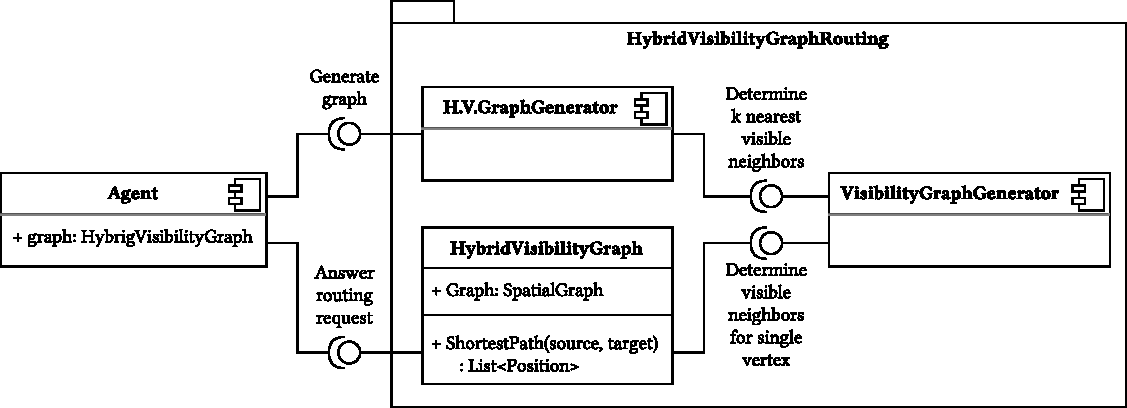
\includegraphics[width=\textwidth]{images/components.pdf}
		\end{figcenter}
		\caption{The components and usages of interfaces of the resulting implementation.}
		\label{fig:components}
	\end{figure}
	
	The first step for a consumer of the system, e.g. an agent based simulation, is to generate the hybrid visibility graph.
	Hence, the \texttt{HybridVisibilityGraphGenerator} (abbreviated as \enquote{H.V.GraphGenerator} in \cref{fig:components}) presents a public interface for this task.
	The result of the graph generation is an instance of the \texttt{HybridVisibilityGraph} class offering public methods to answer shortest path requests, such as the \texttt{ShortestPath} method returning a list of positions (i.e. coordinates) representing the shortest path between two input coordinates.
%	More details on the graph generation can be found in \cref{sec:graph-generation}.
	
	For convenience and due to required preparations, routing queries are put to the hybrid visibility graph.
	To fulfill the overall concept of this work, it must be possible to start and end at arbitrary locations, thus, there is no guarantee that the source and destination locations of the query are on any vertex in the graph.
	Therefore, the hybrid visibility graph has to temporarily connect these locations to the graph.
	This is done by determining all visible neighbors of the source and destination locations and then merging the resulting edges to the underlying graph.
	To perform this task, the hybrid visibility graph uses the interface of the \texttt{VisibilityGraphGenerator} to determine visibility neighbors of a single vertex.
	\Cref{sec:answering-queries} covers the process of answering routing queries in more details, including the clean up step that is performed after the shortest path has been found.

\section{Deployment view}

	% published in MARS

